\documentclass{article}
\usepackage{listings}
\usepackage{graphicx}
\usepackage{fancyhdr}
\usepackage{xcolor}

\definecolor{codegreen}{rgb}{0,0.6,0}
\definecolor{codegray}{rgb}{0.5,0.5,0.5}
\definecolor{codepurple}{rgb}{0.58,0,0.82}
\definecolor{backcolour}{rgb}{0.95,0.95,0.92}

% \lstdefinestyle{mystyle}{
%   backgroundcolor=\color{backcolour}, commentstyle=\color{codegreen},
%   keywordstyle=\color{magenta},
%   numberstyle=\tiny\color{codegray},
%   stringstyle=\color{codepurple},
%   basicstyle=\ttfamily\footnotesize,
%   breakatwhitespace=false,         
%   breaklines=true,                 
%   captionpos=b,                    
%   keepspaces=true,                 
%   numbers=left,                    
%   numbersep=5pt,                  
%   showspaces=false,                
%   showstringspaces=false,
%   showtabs=false,                  
%   tabsize=2
% }

% \lstset{style=mystyle}
\lstset{basicstyle=\ttfamily,
  showstringspaces=false,
  commentstyle=\color{red},
  keywordstyle=\color{blue}
}



\title{CS108 Bash Grader Testcases and Explanation}
\author{Aditya Neeraje : 23B0940}
\date{April 28, 2024}
\graphicspath{{./Images/}}

\begin{document}
    \maketitle
    \clearpage
    \section{Initialize}
    Running the following command initializes 4 csv files with random data and combines some of this data into main.csv.
    \begin{lstlisting}[language=bash]
        python3 initialize.py
    \end{lstlisting}
    \begin{figure}[htbp]
        \centering
        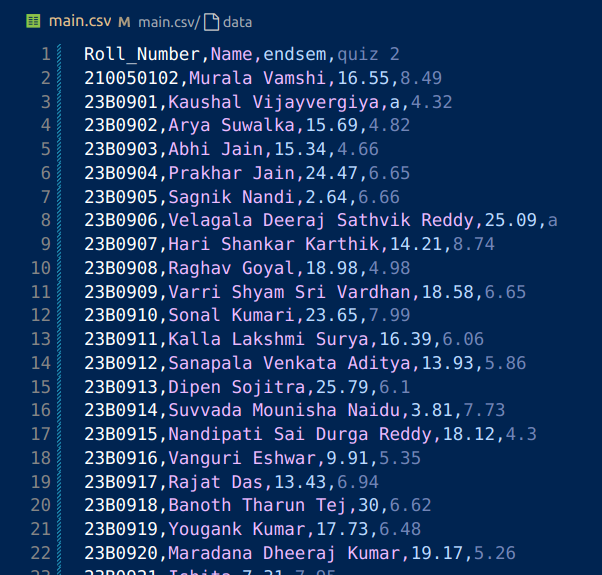
\includegraphics[width=0.4\textwidth]{Initialize}
        \caption{main.csv after Initializing}
        \label{fig:initialize}
    \end{figure}

    \section{Combine}
    Running the following command combines the data from 4 csv files into main.csv.
    \begin{lstlisting}[language=bash]
        bash submission.sh combine
    \end{lstlisting}
    \begin{figure}[htbp]
        \centering
        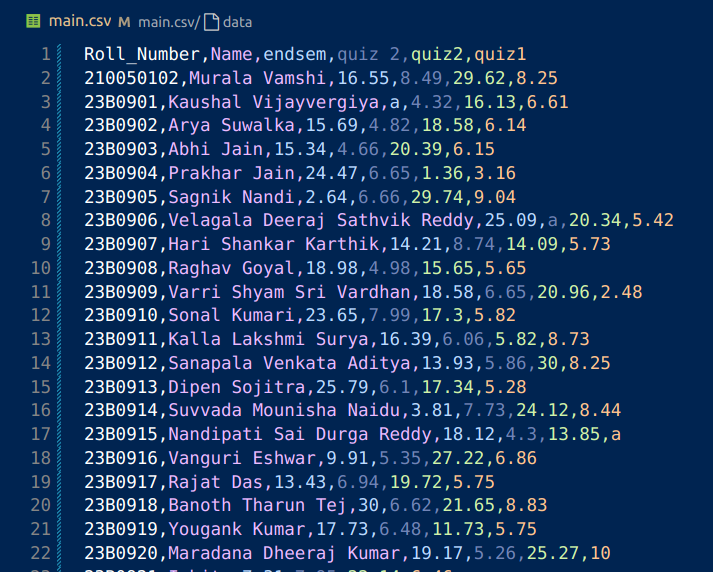
\includegraphics[width=0.4\textwidth]{Combine_all}
        \caption{main.csv after combining all 4}
        \label{fig:combine_all}
    \end{figure}

    You can specify files to drop by passing them as arguments to the script.
    \begin{lstlisting}[language=bash]
        bash submission.sh combine --drop quiz1.csv "quiz 2.csv"
        bash submission.sh combine -d quiz1.csv "quiz 2.csv"
    \end{lstlisting}
    \begin{figure}[htbp]
        \centering
        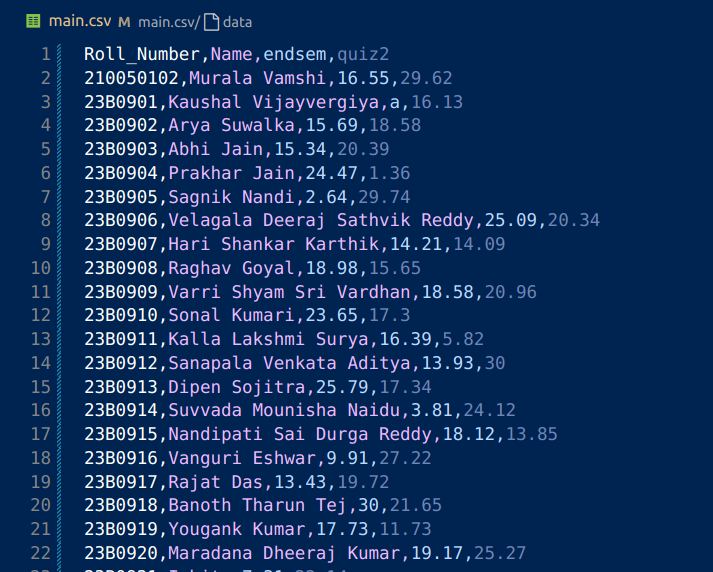
\includegraphics[width=0.4\textwidth]{Drop_two_quizzes}
        \caption{main.csv after dropping quiz1.csv and quiz 2.csv}
        \label{fig:combine_drop}
    \end{figure}

    You can selectively combine back certain quizzes alone by passing them as arguments before any other flag.
    \begin{lstlisting}[language=bash]
        bash submission.sh combine quiz1.csv
    \end{lstlisting}
    \begin{figure}[htbp]
        \centering
        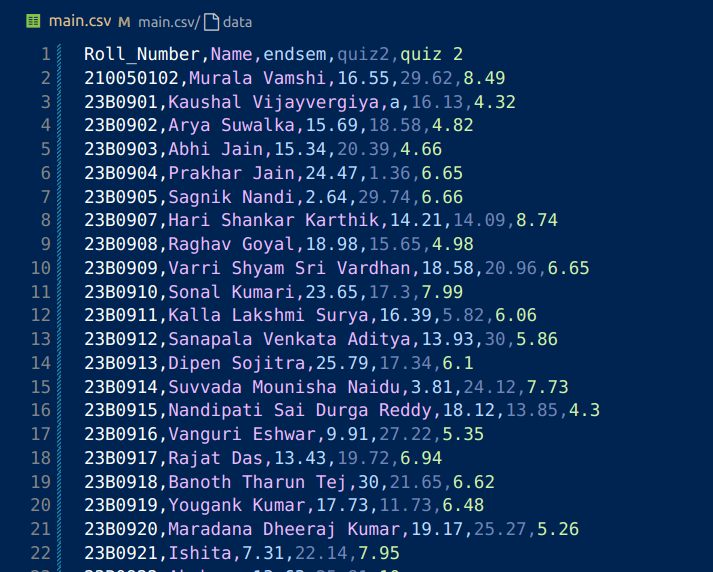
\includegraphics[width=0.4\textwidth]{Combine_quiz_2.png}
        \caption{main.csv after combining quiz 2.csv}
        \label{fig:combine_quiz1}
    \end{figure}

    Generally, combine does not recheck or recombine quizzes which already have a column assigned to them in main.csv, and whose first 3 lines of data are valid marks. Use the --force flag to combine them.
    \begin{lstlisting}[language=bash]
        bash submission.sh combine quiz1.csv quiz2.csv "quiz 2.csv" --force
    \end{lstlisting}
    \begin{figure}[htbp]
        \centering
        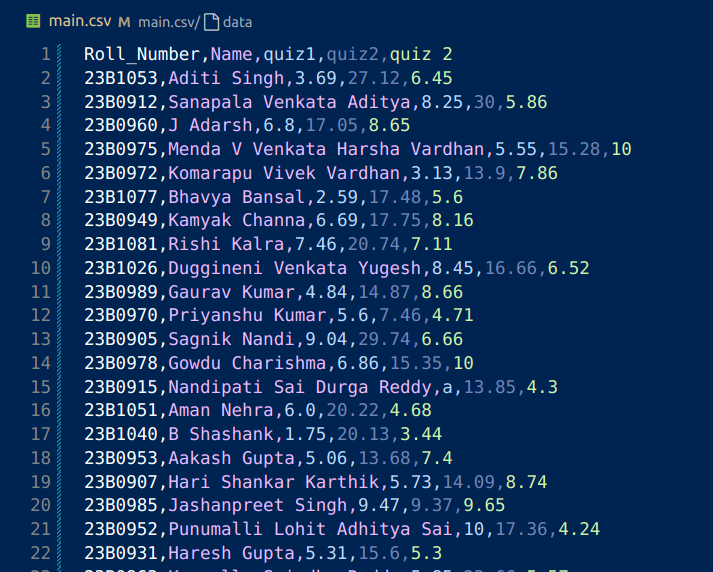
\includegraphics[width=0.4\textwidth]{Force_flag}
        \caption{main.csv after combining all but endsem with force}
        \label{fig:combine_quiz1_force}
    \end{figure}
    Note here that endsem.csv is actually lost from main, since both the force\_flag and the only\_flag are true and endsem.csv is not amongst the list of quizzes to only add to main.
        
\end{document}